\section{Teori}

\subsection{Formål og bakgrunn}

Formålet med denne laboratorieøvelsen er å undersøke hvordan dioder oppfører seg i ulike elektroniske kretser ved vekselspenning (AC). Dette inkluderer analyse av både vanlige dioder og zenerdioder, samt deres anvendelse i klippekretser og likeretterkretser.
\\[1em]
Videre er hensikten å oppnå forståelse for hvordan dioder kan brukes til å forme og omdanne signaler, herunder enveis og toveis likeretting, samt spenningsbegrensning ved hjelp av klippekretser.
\\[1em]
Det legges også vekt på å sammenligne teoretiske beregninger med praktiske målinger ved bruk av oscilloskop og multimeter, og dermed vurdere avvik mellom ideelle modeller og virkelige komponenter.

\subsection{Teoretisk grunnlag i grunnleggende kretsanalyse}
Før vi kan analysere dioder og deres anvendelser, er det viktig å forstå grunnleggende prinsipper for kretsanalyse, inkludert Ohms lov og Kirchhoffs lover. Disse prinsippene danner grunnlaget for å kunne beregne strøm, spenning og effekt i elektriske kretser, og er essensielle for å kunne forstå hvordan dioder påvirker kretsens oppførsel.

\subsubsection{Ohms lov}
Ohms lov beskriver sammenhengen mellom spenning (V), strøm (I) og motstand (R) i en elektrisk krets. Loven sier at strømmen gjennom en metallisk leder med konstant temperatur er proporsjonal med den elektriske potensialforskjellen (spenningen) over lederen, og omvendt proporsjonal med motstanden. Matematisk uttrykkes dette som:
\begin{equation}
    V = I \cdot R
\end{equation}
\noindent
hvor $I$ er strømmen gjennom lederen målt i ampere (A), $V$ er spenningen over lederen målt i volt (V), og $R$ er motstanden til lederen målt i ohm ($\Omega$). Kretsen under viser en enkel krets der alle størrelsene inngår.

\begin{figure}[H]
\centering
\begin{circuitikz}[american voltages]
    \node[circle, draw=black, fill=none, thick, inner sep=2pt] (A) at (-1,2) {};
    \node[circle, fill=black, inner sep=0pt] (B) at (1,2) {};
    \node[circle, fill=black, inner sep=0pt] (C) at (1,-2) {};
    \node[circle, draw=black, fill=none, thick, inner sep=2pt] (D) at (-1,-2) {};

    \node at (-1, 1.6) {$+$};
    \node at (-1, -1.6) {$-$};
    \node at (-1, 0) {$V$};

    \draw (A) to[short, -, i^=$I$] (B);
    \draw (B) to[R=$R$] (C);
    \draw (C) to[short, -] (D);

\end{circuitikz}
\caption{Illustrasjon av Ohms lov i en enkel krets.}
\label{fig:ohm}
\end{figure}

\paragraph{Anvendelse i kretsanalyse. } Ohms lov utgjør grunnlaget for analyse i elektriske kretser. Loven benyttes sammen med andre lover for å bestemme ukjente strømmer, spenninger og motstander i komplekse kretser. I kretser med dioder vil Ohms lov være verktøyet for å kunne beregne strøm og spenninger for å få et teoretisk grunnlag for å kunne sammenligne med praktiske målinger.

\subsubsection{Kirchhoffs lover}
Kirchhoffs lover består av to grunnleggende prinsipper for elektriske kretser: \textbf{Kirchhoffs strømlov} (KCL) og \textbf{Kirchhoffs spenningslov} (KVL). Disse lovene beskriver konservering av elektrisk ladning og energi, og er essensielle for å kunne analysere og forstå komplekse kretser, inkludert de som inneholder dioder. 

\paragraph{Kirchhoffs strømlov (KCL). } Denne loven beskriver konservasjon av elektrisk ladning. KCL sier at summen av strømmer som kommer inn i et nodepunkt i en elektrisk krets, er lik summen av strømmer som går ut av det samme nodepunktet.

\begin{figure}[H]
\centering
\begin{circuitikz}[american voltages]
    \node[circle, fill=black, inner sep=1.2pt] (A) at (0, 0) {};
    \node[circle, fill=black, inner sep=0pt] (B) at (0, 3) {};
    \node[circle, fill=black, inner sep=0pt] (C) at (3, 0) {};
    \node[circle, fill=black, inner sep=0pt] (D) at (0, -3) {};
    \node[circle, fill=black, inner sep=0pt] (E) at (-3, 0) {};


    \draw (A) to[R=$R_1$, i^=$i_1$] (B);
    \draw (C) to[R=$R_2$, i^=$i_2$] (A);
    \draw (D) to[R=$R_3$, i^=$i_3$] (A);
    \draw (A) to[R=$R_4$, i^=$i_4$] (E);
    

\end{circuitikz}
\caption{Illustrasjon av et forgreningspunkt med inn- og utgående strømmer.}
\label{fig:KCL}
\end{figure}

\[
\sum_{n=1}^{N} I_n = 0
\]
\\[1em]
\noindent
I figur~\ref{fig:KCL} vil KCL kunne uttrykkes som:
\[
i_2 + i_3 - i_1 - i_4 = 0
\]

\paragraph{Kirchhoffs spenningslov (KVL). } Denne loven beskriver konservasjon av elektrisk energi. KVL sier at summen av alle elektriske potensialendringer (spenninger) rundt en lukket sløyfe i en elektrisk krets, er lik null. I en sløyfe med $N$ forgreninger med spenninger $V_n$, kan KVL uttrykkes som:

\[
\sum_{n=1}^{N} V_n = 0
\]
\\[1em]
\noindent
Kretsen i figur~\ref{fig:KVL} viser en sløyfe med fire elementer. Ved å følge retningen av den elektriske strømmen, kan KVL uttrykkes som:
\[
-V_4 + V_1 + V_2 + V_3 = 0
\]

\begin{figure}[H]
\centering
\begin{circuitikz}[american voltages]
    \node[circle, fill=black, inner sep=0pt] (A) at (-3, 2.5) {};
    \node[circle, fill=black, inner sep=0pt] (B) at (3, 2.5) {};
    \node[circle, fill=black, inner sep=0pt] (C) at (3, -2.5) {};
    \node[circle, fill=black, inner sep=0pt] (D) at (-3, -2.5) {};


    \draw (A) to[R=$R_1$, v_=$V_1$] (B);
    \draw (B) to[R=$R_2$, v_=$V_2$] (C);
    \draw (C) to[R=$R_3$, v_=$V_3$] (D);

    \draw (A) to[V=$V_4$] (D);

    \draw[->] (0, -1) arc[start angle=-90,end angle=-360,radius=1];

    \node at (0, 0) {$I$};

\end{circuitikz}
\caption{Illustrasjon av en sløyfe.}
\label{fig:KVL}
\end{figure}

\subsection{Dioder}
En diode er en to-terminal elektrisk komponent som leder elektrisk strøm primært i en retning. Dioden har lav motstand (ideellt null) i en retning og høy motstand (ideellt uendelig) i den motsatte retningen. Formålet med dioden i applikasjoner og kretser er å kontrollere retningen av elektrisk strøm~\cite{wikipediaDiodes}.

\begin{figure}[H]
\centering
\begin{circuitikz}[american voltages]
    \node[circle, fill=black, inner sep=0pt] (A) at (-2, 0) {};
    \node[circle, fill=black, inner sep=0pt] (B) at (2, 0) {};

    \draw (A) to[D, v_=$V_D$, i^=$I_D$] (B);

  \end{circuitikz}
\caption{Symbolet for diode i kretser.}\label{fig:Diode}
\end{figure}

\paragraph{Diodens oppbygning. } For å oppnå formålet med en diode, er den konstruert med en p-n-overgang. Dette betyr at dioden består av to halvledere, en type \textbf{p (positiv)} og en type \textbf{n (negativ)}. Dette er oppnådd ved å \textbf{dope} et halvledermateriale. Doping er prosessen hvor meget rene halvledere tilsettes kontrollerte mengder av urenheter. Dette påvirker krystallstrukturen til stoffet. I en p-type halvleder er det et overskudd av hull (positive ladningsbærere), mens i en n-type halvleder er det et overskudd av elektroner (negative ladningsbærere)~\cite{wikipediaDoping}. Katoden er den negative terminalen i en diode, og anoden er den positive terminalen.
\\[1em]
Ser vi på en silisiumsdiode med silisiumsstruktur, vil doping av silisium med fosfor (P) skape en n-type halvleder, hvor det er et overskudd av elektroner. Disse ekstra elektronene er frie til å bevege seg gjennom krystallstrukturen. Doper vi silisium med bor (B), vil det skape en p-type halvleder, hvor det er et overskudd av hull. Disse hullene fungerer som positive ladningsbærere~\cite{learningBook}.

\begin{figure}[H]
\centering

\begin{subfigure}{0.45\textwidth}
\centering
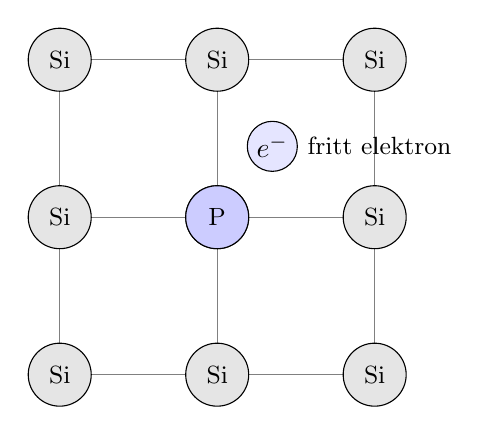
\begin{tikzpicture}
% --- N-TYPE ---
 % bonds
  \draw[gray] (0,0) -- (2,0) -- (4,0);
  \draw[gray] (0,2) -- (2,2) -- (4,2);
  \draw[gray] (0,4) -- (2,4) -- (4,4);
  \draw[gray] (0,0) -- (0,2) -- (0,4);
  \draw[gray] (2,0) -- (2,2) -- (2,4);
  \draw[gray] (4,0) -- (4,2) -- (4,4);

  % silicon lattice
  \foreach \x in {0,2,4} {
    \foreach \y in {0,2,4} {
      \node[draw, circle, fill=gray!20, minimum size=8mm] at (\x,\y) {\small Si};
    }
  }

  % dopant atom
  \node[draw, circle, fill=blue!20, minimum size=8mm] at (2,2) {\small P};

  % extra electron
  \node[draw, circle, fill=blue!10, inner sep=1.5pt, label=right:{\small fritt elektron}] at (2.7,2.9) {$e^-$};
\end{tikzpicture}
\caption{n-type doping}
\end{subfigure}
\hfill
\begin{subfigure}{0.45\textwidth}
\centering
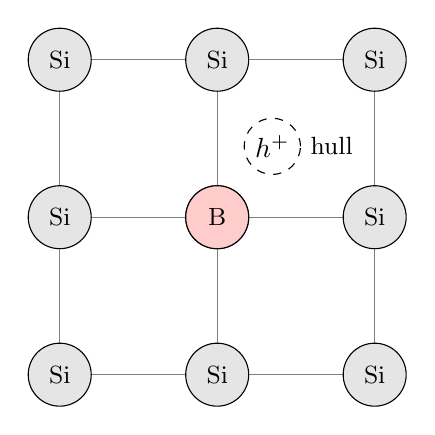
\begin{tikzpicture}
% --- P-TYPE ---
% bonds
  \draw[gray] (0,0) -- (2,0) -- (4,0);
  \draw[gray] (0,2) -- (2,2) -- (4,2);
  \draw[gray] (0,4) -- (2,4) -- (4,4);
  \draw[gray] (0,0) -- (0,2) -- (0,4);
  \draw[gray] (2,0) -- (2,2) -- (2,4);
  \draw[gray] (4,0) -- (4,2) -- (4,4);

    % silicon lattice
\foreach \x in {0,2,4} {
    \foreach \y in {0,2,4} {
      \node[draw, circle, fill=gray!20, minimum size=8mm] at (\x,\y) {\small Si};
    }
  }

  % dopant atom
  \node[draw, circle, fill=red!20, minimum size=8mm] at (2,2) {\small B};

  % hole
  \node[draw, circle, dashed, inner sep=2pt, label=right:{\small hull}] at (2.7,2.9) {$h^+$};
\end{tikzpicture}
\caption{p-type doping}
\end{subfigure}

\caption{Illustrasjon av doping i halvledere}
\end{figure}

\noindent
Disse materialene er satt sammen i en p-n-overgang for å danne en diode. Elektronene og hullene vil diffundere over grenseflaten mellom de to materialene. Dette skaper et område kalt \textbf{deplasjonsregionen}, hvor det er en elektrisk felt som hindrer videre diffusjon av ladningsbærere. Når en spenning påføres i fremoverretning (positiv spenning på anoden), vil dette elektriske feltet reduseres, og dioden vil etter nok spenningsforskjell over dioden, begynne å lede strøm. Når en spenning påføres i revers retning (positiv spenning på katoden), vil det elektriske feltet øke, og dioden vil ikke lede strøm, bortsett fra en liten lekkasjestrøm. Denne lekkasjestrømmen er vanligvis ubetydelig og blir ikke tatt høyde for i teoretiske beregninger~\cite{learningBook}.

\paragraph{Diodens karakteristiske kurve. } Diodens karakteristiske kurve viser forholdet mellom strømmen gjennom dioden og spenningen over den. I fremoverretning vil strømmen øke eksponentielt etter at en terskelspenning (for silisiumdiode, ca. 0.7 V) er nådd. I revers retning vil strømmen være svært liten (lekkasjestrøm) inntil en viss spenning, kalt brytespenningen, hvor dioden begynner å lede i revers retning~\cite{wikipediaDiodes}.

\begin{figure}[H]
\centering

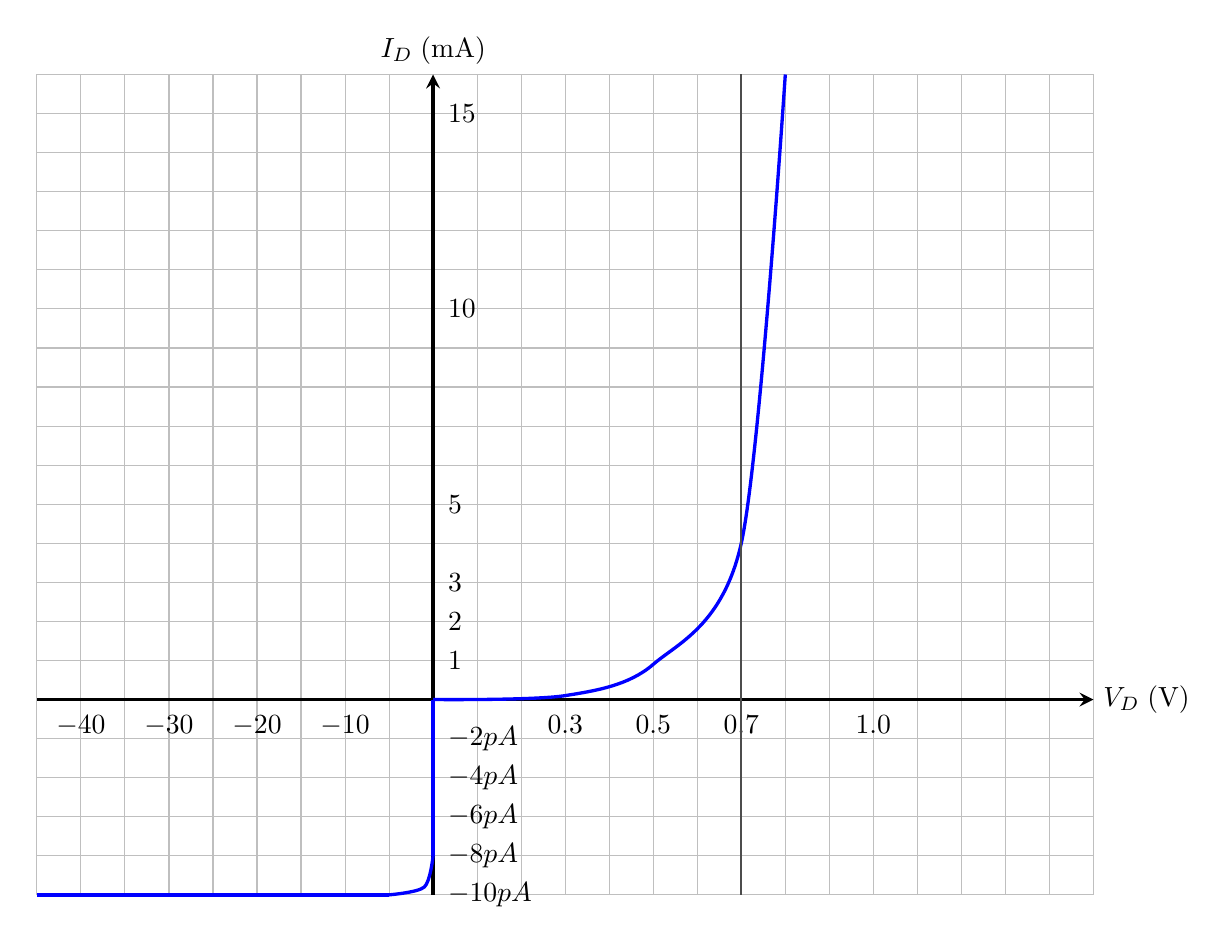
\begin{tikzpicture}
\begin{axis}[
    width=15cm,
    height=12cm,
    xmin=-9, xmax=15,
    ymin=-5, ymax=16,
    axis lines=middle,
    axis line style={black, very thick},
    xlabel={$V_D\;(\mathrm{V})$},
    ylabel={$I_D\;(\mathrm{mA})$},
    xlabel style={at={(current axis.right of origin)}, anchor=west},
    ylabel style={at={(current axis.above origin)}, anchor=south},
    xtick={-9,-8,...,15},
    xticklabels={
    {}, $-40$, {}, $-30$, {}, $-20$, {}, $-10$, {}, $0$,
    {}, {}, $0.3$, {}, $0.5$, {}, $0.7$, {}, {}, $1.0$, {}, {}, {}, {}
    },
    ytick={-5,-4,...,16},
    yticklabels={$-10\unit{pA}$, $-8\unit{pA}$, $-6\unit{pA}$, $-4\unit{pA}$, $-2\unit{pA}$, $0$, $1$, $2$, $3$, {}, $5$, {}, {}, {}, {}, $10$, {}, {}, {}, {}, $15$, {},},
    yticklabel style={xshift=4pt, anchor=west},
    grid=both,
    major grid style={gray!50, line width=0.4pt},
    minor grid style={gray!30, line width=0.2pt},
    tick style={draw=none},
    minor tick num=0,
    enlargelimits=false,
    clip=false
]

\addplot[
    blue,
    very thick,
    smooth
] coordinates {
    (0,0)
    (3,0.1)
    (5,0.9)
    (7,4)
    (8,16)
};

\addplot[
    blue,
    very thick,
    smooth
] coordinates {
    (-1,-5)
    (-0.2, -4.8)
    (0,-4)
};

\addplot[
    blue,
    very thick
] coordinates {
    (-9,-5)
    (-1,-5)
};

\addplot[
    blue,
    very thick
] coordinates {
    (0,-4)
    (0,0)
};

\draw[black!70, thick] (axis cs:7,-5) -- (axis cs:7,16);

\end{axis}
\end{tikzpicture}

\caption{Silisiumdiodes karakteristiske kurve~\cite{learningBook}.}\label{fig:silisiumsDiodeKurve}
\end{figure}

\noindent
Diodens karakteristiske kurve viser sammenhengen mellom spenninngen over dioden ($V_D$) og strømmen gjennom dioden ($I_D$). Kurven gir oss dermed en rekke arbeidspunkter for dioden. Om en gitt spenning er påført dioden, kan vi finne den tilsvarende strømmen ved å se på kurven. Kurven for silisiumsdioder i figur~\ref{fig:silisiumsDiodeKurve} viser at i fremoverretning, etter at terskelspenningen på ca. 0.7 V er nådd, øker strømmen kraftig. I revers retning er strømmen svært liten (lekkasjestrøm). For teoretiske beregninger i denne rapporten vil 0.7 V brukes som terskelspenning for silisiumsdioder.

\subsubsection{Zenerdioder}

En zenordiode er en spesiell type diode som er designet for å lede strøm i revers retning når en bestemt spenning, kalt zenerspenningen, er nådd. Siden zenerdioder er konstruert for å operere i revers brudd, har de en karakteristisk kurve som viser at når zenerspenningen er nådd, vil strømmen øke kraftig i revers retning. Zenerdioder brukes ofte i spenningsregulatorer og beskyttelseskretser for å sikre at spenningen ikke overstiger et bestemt nivå~\cite{wikipediaZenerDiodes}.

\begin{figure}[H]
\centering
\begin{circuitikz}[american voltages]
    \node[circle, fill=black, inner sep=0pt] (A) at (-2, 0) {};
    \node[circle, fill=black, inner sep=0pt] (B) at (2, 0) {};

    \draw (A) to[zzD, v_=$V_D$, i^=$I_D$] (B);

  \end{circuitikz}
\caption{Symbolet for zenerdiode i kretser.}\label{fig:ZenerDiode}
\end{figure}

\noindent
I figur~\ref{fig:ZenerDiode} vil zenordioden teoretisk lede strøm dersom $V_D > 0.7\text{V}$. Zenordioden vil også lede strøm i revers retning dersom $V_D < -V_Z$, hvor $V_Z$ er zenerspenningen.
\paragraph{Zenordiodens karakteristiske kurve. } Denne er lik den for en vanlig diode for $V_D > 0.7\text{V}$. For $V_D < 0\text{V}$ vil dioden etter gjennombruddsspenning (zenorspenning) øke ledet strøm kraftig.

\begin{figure}[H]
\centering

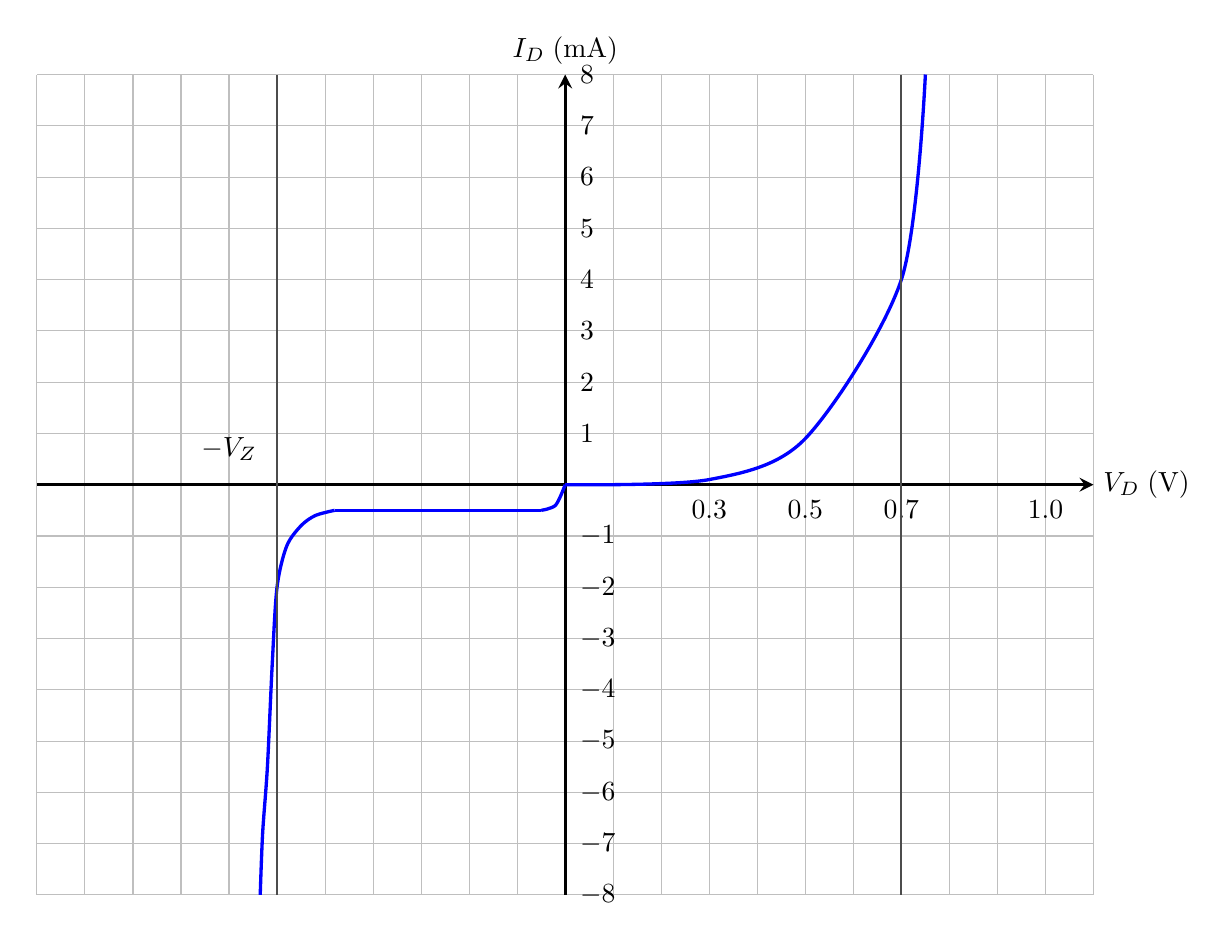
\begin{tikzpicture}
\begin{axis}[
    width=15cm,
    height=12cm,
    xmin=-11, xmax=11,
    ymin=-8, ymax=8,
    axis lines=middle,
    axis line style={black, very thick},
    xlabel={$V_D\;(\mathrm{V})$},
    ylabel={$I_D\;(\mathrm{mA})$},
    xlabel style={at={(current axis.right of origin)}, anchor=west},
    ylabel style={at={(current axis.above origin)}, anchor=south},
    xtick={-11,-10,...,11},
    xticklabels={
    {}, {}, {}, {}, {}, {}, {}, {}, {}, {}, {}, $0$,
    {}, {}, $0.3$, {}, $0.5$, {}, $0.7$, {}, {}, $1.0$, {}, {}, {}, {}
    },
    ytick={-8,-7,...,8},
    yticklabel style={xshift=4pt, anchor=west},
    grid=both,
    major grid style={gray!50, line width=0.4pt},
    minor grid style={gray!30, line width=0.2pt},
    tick style={draw=none},
    minor tick num=0,
    enlargelimits=false,
    clip=false
]

\addplot[
    blue,
    very thick,
    smooth
] coordinates {
    (0,0)
    (3,0.1)
    (5,0.9)
    (7,4)
    (7.5,8)
};

\addplot[
    blue,
    very thick,
    smooth
] coordinates {
    (-0.5,-0.5)
    (-0.2, -0.4)
    (0,0)
};

\addplot[
    blue,
    very thick
] coordinates {
    (-4.8,-0.5)
    (-0.5,-0.5)
};

\addplot[
    blue,
    very thick,
    smooth
] coordinates {
    (-4.8, -0.5)
    (-5.2, -0.6)
    (-5.5, -0.8)
    (-5.8, -1.2)
    (-6.0, -2.0)
    (-6.1, -3.5)
    (-6.2, -5.5)
    (-6.3, -6.8)
    (-6.35, -8.0)
};

\node at (-7, 0.7) {$-V_Z$};

\draw[black!70, thick] (axis cs:7,-8) -- (axis cs:7,8);

\draw[black!70, thick] (axis cs:-6,-8) -- (axis cs:-6,8);

\end{axis}
\end{tikzpicture}

\caption{Zenerdiodes karakteristiske kurve~\cite{learningBook}.}\label{fig:zenerdiodeKurve}
\end{figure}

\noindent
Zenordiodens karakteristiske kurve i figur~\ref{fig:zenerdiodeKurve} viser at den er lik en vanlig diodes karakteristiske kurve for $V_D > 0.7\text{V}$. For $V_D < 0\text{V}$ vil dioden etter gjennombruddsspenning (zenorspenning) øke ledet strøm kraftig i revers retning. Dioden lekker også noe strøm ved alle negative spenninger, men i teoretiske beregninger i denne rapporten vil dette ikke tas høyde for. I tillegg kan vi se at kurven blir nærmest vertikal ved $V_D = -V_Z$, noe som indikerer at dioden vil lede en stor strøm for små endringer i spenning rundt zenerspenningen, og at spenningen er nærmest konstant. Dette gjør zenerdioden spesielt nyttig for spenningsregulering, da den kan opprettholde en stabil spenning over seg selv til tross for variasjoner i strømmen som går gjennom den~\cite{wikipediaZenerDiodes}.

\subsection{Klippekretser}
Klippekretser er kretser som bruker dioder for å ``klippe'' eller begrense spenningen i en krets til et bestemt nivå. Dette kan være nyttig for å beskytte komponenter mot overspenning eller for å forme signaler. Klippekretser kan være enveis eller toveis, avhengig av om de begrenser spenningen i én retning eller begge retninger~\cite{wikipediaClippers}.
\\[1em]
Klippekretsen konstrueres ved å plassere en diode i serie med en motstand, og deretter koble denne kombinasjonen i parallell med lasten. Bruker vi en vanlig diode, vil klippekretser begrense spenningen i fremover retning på 0.7V. Bruker vi en zenerdiode, kan vi begrense spenningen i både fremover på 0.7V og revers retning på zenorspenningen~\cite{wikipediaClippers}.
\\[1em]

\begin{figure}[H]
\centering
\begin{circuitikz}
\draw
(0,0) to[sV, l={$V_{in}(t)$}] (0,3)
      to[R, l=$R$] (5,3)
      to[D] (5,0)
      to[short] (0,0);

\node[circle, draw=black, fill=none, thick, inner sep=2pt] (Vtop) at (7,3) {};
\node[circle, draw=black, fill=none, thick, inner sep=2pt] (Vbot) at (7,0) {};

\draw (5,3) to[short] (Vtop) node[below] {$+$};
\draw (5,0) to[short] (Vbot) node[above] {$-$};

\node at (7, 1.5) {$V_{out}(t)$};


\node at (0, 0)[ground] {};
\end{circuitikz}
\caption{Klippekrets bestående av motstand og diode som begrenser utgangsspenningen.}
\label{fig:clipper_circuit}
\end{figure}

\begin{figure}[H]
\centering
\begin{tikzpicture}
\begin{axis}[
    width=11cm,
    axis lines=middle,
    xlabel={$t$},
    ylabel={$V$},
    xmin=0, xmax=6.28,
    ymin=-1.2, ymax=1.2,
    samples=200,
    domain=0:6.28,
    ytick={-1,-0.5,0,0.7,1},
    yticklabels={$-1$, $-0.5$, $0$, $0.7$, $1$},
    xtick={3.14,6.28},
    xticklabels={$T/2$, $T$},
    legend style={
        at={(0.98,0.98)},
        anchor=north east,
        draw=none,
        fill=none
    }
]
\addplot[
    blue,
    thick
] {sin(deg(x))};
\addlegendentry{$V_{in}$}

\addplot[
    red,
    thick
] {min(sin(deg(x)), 0.7)};
\addlegendentry{$V_{out}$}

\end{axis}
\end{tikzpicture}
\caption{Inngangs- og utgangsspenning for klippekretsen i figur~\ref{fig:clipper_circuit}. Inngangssignalet $V_{in}$ er sinusformet, mens utgangssignalet $V_{out}$ begrenses til omtrent $0.7\,\mathrm{V}$ når dioden leder.}
\label{fig:clipper_in_out}
\end{figure}

\subsection{Likeretting}

\subsubsection{Énveis likeretter}
\subsubsection{Toveis likeretter}
\subsubsection{DC-verdi og rippel}

\subsection{Glatting med kondensator~--~RC-ledd}

\subsection{AC- og DC-måling}
\subsubsection{Oscilloskop}